\scanpage{49}
% E: text|upper left date|2.1.84
2.1.84
% E: text|upper left, cancelled draft opening|On place sur K
\deleted{On place sur \(K\) des nouveaux sommets (d'ordre 2), de la façon suivante; \deleted{Pour \unsure{chaque face (soit \(F\)) du quadrillage, on prend les sommets}} \unsure{points par côté fermé}.

% E: text|upper left, cancelled a and b|On rajoute les pts
\deleted{a) On rajoute les pts de \(K\cap L\) sur \(\delta F\).

b) Pour toute arête du nouveau complexe topologique \((\delta F,S\cap\unsure{\partial F|\delta F}\cup(\delta F\cap L))\), \unsure{on en distingue}}

% E: drawing|left upper-middle, marked edge|s and red orange marks
\figure{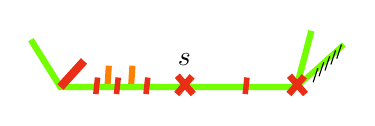
\begin{tikzpicture}[scale=.75]
\draw[green!55!yellow,line width=2.3pt](-.5,.8)--(0,0)--(4,0)--(4.25,.95);\draw[green!55!yellow,line width=2pt](4,0)--(4.8,.72);
\draw[red!65!brown,line width=3pt](0,0)--(.4,.44);
\foreach \x in {.6,.95,1.45,3.13}{\draw[red!65!brown,line width=2pt](\x,-.12)--(\x+.03,.16);}
\foreach \x in {.8,1.2}{\draw[orange,line width=2.2pt](\x,.05)--(\x+.02,.36);}
\foreach \x in {2.1,4}{\draw[red!65!brown,line width=2.4pt](\x-.13,-.12)--(\x+.13,.18);\draw[red!65!brown,line width=2.4pt](\x-.12,.19)--(\x+.15,-.12);}
\node[above]at(2.1,.2){\(s\)};
\foreach \x in {4.28,4.38,4.48,4.58,4.68}{\draw[black](\x,\x-4.2)--(\x+.08,\x-3.96);}
\end{tikzpicture}}

% E: text|upper middle, replacement a|Rajoutons les pts
a) Rajoutons les pts de \(\widehat a\cap L\)
% E: display|upper middle|a' = (a,a intersect S(K) union a intersect L)
\[
-\quad\text{soit }\underline{a}'=(a,a\cap S(K)\cup a\cap L)
\]
% E: text|middle left, structure and NB|Le graphe
\unsure{Le graphe est ainsi structuré}\inserted{top.}, soit \(\alpha\) une arête de ce graphe. (\uline{NB} \deleted{\(\unsure{\xi}\)} Il y a au moins un \deleted{c) Si une des est} élément de \(a\cap L\) (``\deleted{\unsure{arête}}\inserted{sommet} rouge'') sur \(a\) distinct des extrémités, donc chaque arête \(\alpha\) de \(\underline a'\) \deleted{est} a au moins une extrémité rouge, i.e. qui n'est pas une \deleted{sommet}\inserted{extrémité} de \(\underline a\), et il y en a exactement deux qui n'en ont qu'une de rouge (\unsure{c'est les ptés arêtes}).

% E: text|lower left, new a|Sur ces dernières
a) Sur ces dernières, on ne rajoute pas d'autre sommet\inserted{\unsure{sauf si l'extrémité est un sommet de \(L\)}}. \deleted{Sur toutes}\inserted{\unsure{Pour les}} autres arêtes, on \deleted{\unsure{dis}} rajoute des sommets (oranges) de la façon suivante

% E: text|lower left, b|Si les deux extrémités
b) Si \deleted{\unsure{ttes}} les\inserted{deux} extrémités sont non critiques, i.e. ne sont pas des sommets de \(\unsure{L|K}\), on rajoute juste un sommet (le milieu)

% E: text|bottom left, c unfinished|Pour les deux autres arêtes
c) \deleted{Sinon} Pour les deux autres arêtes (cas d'une arête \(\underline a\) ordinaire), de part et d'autre du pt critique \deleted{\(\unsure{\xi}\)} \(s\), si \(\nu(s)\) est un \unsure{ordre|entier}, on dispose \(\frac{\nu(s)}2\) pts \unsure{oranges|rouges} (si
}

% E: drawing|upper right, isolated green angle with red vertex and tick|green angle red cross
\figure{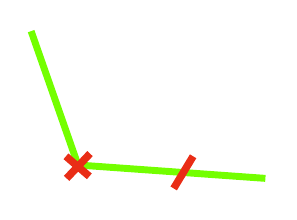
\begin{tikzpicture}[scale=.85]
\draw[green!55!yellow,line width=2.5pt](-.7,2)--(0,0)--(2.8,-.2);
\draw[red!65!brown,line width=2.7pt](-.17,-.2)--(.18,.17);\draw[red!65!brown,line width=2.7pt](-.18,.13)--(.17,-.17);
\draw[red!65!brown,line width=2.7pt](1.43,-.35)--(1.72,.13);
\end{tikzpicture}}
\mspage{48}
